\documentclass{article}

% Language setting
% Replace `english' with e.g. `spanish' to change the document language
\usepackage[english]{babel}

% Set page size and margins
% Replace `letterpaper' with `a4paper' for UK/EU standard size
\usepackage[letterpaper,top=2cm,bottom=2cm,left=3cm,right=3cm,marginparwidth=1.75cm]{geometry}


% Useful packages
\usepackage{amsmath}
\usepackage{graphicx}
\usepackage[colorlinks=true, allcolors=blue]{hyperref}
\usepackage{tikz}
\usepackage{natbib}
\bibliographystyle{unsrtnat}

\usetikzlibrary{shapes.arrows, positioning, arrows.meta}


\title{Theoretical framework}
\author{Riccardo Dal Cero}

\begin{document}
\maketitle

\begin{abstract}
    The main idea is to study how and whether the asymmetry of information have an impact on the cleansing effect of
    recession, replicating the model in computer  simulation.
\end{abstract}

\section[short]{Theoretical framework}
The economy comprises risk-neutral firms with a constant discount rate represented by $0 < \beta < 1$. These firms
exhibit heterogeneity in productivity and net worth. They employ a production technology that relies solely on capital
(or production units) as input, featuring diminishing returns to scale.
\\
In each period, firms incur a fixed production cost denoted as $c$ to initiate production. After production, they decide
how to allocate profits for the next period. The remaining profits are invested in a risk-free asset. Firms face a
choice: they can either continue operating and reinvest their profits or exit the market, investing their entire net
worth, denoted as $e$, in the risk-free asset.
\\
Firms opt to exit the market when expected profits no longer outweigh the fixed cost $c$, or when the value of
production becomes inferior to the value they could gain by investing in the risk-free asset.
\\
The value obtained from investing in the risk-free asset is given by:
\[
q_t + \sum_{s=0}^{+\infty}\beta^s[\beta(1+r)-1]e_{t+s+1}.
\]

Notably, when the condition $\beta(1+r) \leq 1$ holds, this value simplifies to $q$. In such cases, firms are either
indifferent regarding the timing of dividend distributions or have a preference for distributing their end-of-period net
worth to shareholders or investors.
\\
In this economic model, the agents are the firms themselves, aiming to maximize their value over time by selecting an
optimal level of capital denoted as $k$. The production function, accounting for the fixed cost $c$, is expressed as
follows: $Y = Z(\theta + \epsilon)k^\alpha$.
\\
Key variables include:
\begin{itemize}
    \item $Z$: Stochastic aggregate productivity common across firms.
    \item $\theta$: Persistent firm-specific productivity shock (modeled as a Markov Chain).
    \item $\epsilon$: Firm-specific productivity shock with $\epsilon \sim \mathcal{N}(0,\delta)$.
    \item $k^\alpha$: Capital or production units, as in Caballero and Hammour (AER).
\end{itemize}

The timeline of events is as follows:

\begin{figure}[h]
    \centering
    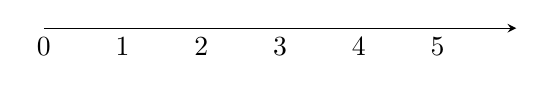
\begin{tikzpicture}
        % Draw timeline
        \draw[->,>=stealth] (0,0) -- (6,0);
        
        % Add timeline labels
        \foreach \x/\label in {0,1, 2,3, 4, 5} {
            \node[align=center, below] at (\x,0) {\label};
        }
    \end{tikzpicture}
    \caption{Timeline of Events}
\end{figure}

The sequence of events includes:
\begin{enumerate}
    \item The firm possesses knowledge of $Z,\theta,k^\alpha,e$ (where $e$ represents its endowment, different from $k$ since the firm can borrow money with $d=c+k-e$).
    \item The firm computes the optimal $k$ to maximize the expected value of the firm, with $k$ ranging from $[0,+\infty]$. If $k=0$, it indicates the firm's decision to exit.
    \item At the end of the period, the firm observes $\epsilon$ and the aggregate shock.
    \item The firm repays its debt and the fixed operating cost $(c+k-e)$, resulting in an end-of-period net worth $q$.
    \item The firm decides on the amount of dividends to distribute $(q-e')$, observes the productivity shock $\theta', Z'$, and the process restarts from step 1.
\end{enumerate}

\subsection{Frictionless economy}
In a frictionless economy, firms have the option to borrow an amount denoted as \(c+k-e\) at the risk-free interest rate
\(r=\frac{1}{\beta}-1\). Therefore, at the start of the period, the firm's value is determined by the following
expression:

\[V_{FL} = \max_{k} E \int \max[q,\max_{e'}(q - e' + \beta V_{FL}(e',\theta', Z'))]  \,d\Phi
(\epsilon) \]
where the end of period net worth is equal to:
\[q=Z(\theta+\epsilon)k^\alpha + (1-\delta )k-(1+r)(c+k-e)\]

Under the condition of survival, it can be demonstrated that:

\[\widehat{V}_{FL}(\theta,Z) = \max_{k}E\int[Z(\theta+\epsilon)k^\alpha - (1+r)c\,d\Phi (\epsilon)] +
\beta\max[0,\widehat{V}_{FL}(\theta',Z')]\]

In the absence of market frictions, firms choose to exit when their productivity reaches a certain threshold.
Specifically, they exit if \(\theta'<\underline{\theta} _{FL}(Z')\), where \(\underline{\theta}
_{FL}(Z')\) is defined as the value
for which \(\widehat{V}_{FL}(\underline{\theta}_{FL},Z')=0\).

\subsection{Economy with Credit Market Frictions}

After production, the firm privately observes the temporary shock $\epsilon$, while financial intermediaries can only
observe it at a cost of $\mu k^\alpha$. For one-period debt contracts, financial intermediaries observe $\epsilon$ only
if the firm faces financial distress, which occurs when the private shock is insufficient to repay its debt. The terms
of the financial contract depend on the firm's net worth $e$, current productivity $\theta$, and aggregate productivity
value $Z$, all observable by both the financial intermediary and the firm at no additional cost.

\textbf{HP1 (Hypothesis 1):} The risk-free interest rate is $\beta < \frac{1}{1+r}$, which implies a lower risk-free
rate in an economy with credit frictions compared to a frictionless one. It also ensures that firms do not always
reinvest their profits.

When a firm defaults, the financial intermediary incurs verification costs and seizes all of the firm's income. The
default threshold $\overline{\epsilon}$ is determined by the equation:
\[
Z(\theta+\overline{\epsilon})k^\alpha + (1-\delta)k = (1+\widetilde{r} )(c+k+e)
\]

Default results in a zero net worth but does not necessarily force the firm to exit the market, depending on its
persistent productivity component $\theta$.

The financial intermediary lends $(c + k - e)$ to the firm only if the expected income from the loan equals the
opportunity cost of the funds, as expressed by the inequality:
\[
(1+\widetilde{r} )(k+c+e)(1-\Phi(\overline{\epsilon}))+\int_{-\infty}^{\overline{\epsilon}}[Z(\theta+\overline{\epsilon})
k^\alpha+(1-\delta)k-\mu k^\alpha] \,d\Phi(\epsilon) \geq (1+r)(c+k+e)
\]

The financial contract is characterized by $(k,\overline{\epsilon})$. Given $Z,\theta,e$, the participation constraint
indicates the default threshold $\overline{\epsilon}$ required by the financial intermediary to lend a given amount. For
some firms, their net worth is too low for the participation constraint of the financial intermediary to be satisfied.
In fact, given $\theta, Z$, there is a unique threshold $e_b(\theta,Z)$ below which the financial intermediary
refuses to lend any amount:
\[
Z[\theta+G(\overline{\epsilon}_b )]k^\alpha+(1-\delta)k-uk_b^\alpha\Phi (\overline{\epsilon}_b)=(1+r)(k_b+c-\underline{e_b})
\]
where $\overline{\epsilon}_b$ maximizes the expected income of the financial intermediary. When the firm has a net worth
below $\underline{e_b}$, the firm defaults.

After production, the firm's end-of-period net worth is equal to:
\[
q = \begin{cases}
  Z(\theta+\overline{\epsilon})k^\alpha +(1-\delta)k-(1+\widetilde{r})(k+c-e) & \text{if } \epsilon\geq \overline{\epsilon} \\
  0 & \text{otherwise}
\end{cases}
\]
Using the default condition we can rewrite as 
\[q = \max[Zk^\alpha(\epsilon-\overline{\epsilon});0]\]

\subsection{The firm's problem}
Define $V$ as the firm's value at the start of the period, which hinges on investment outcomes and exit decisions. If
the end-of-period net worth falls below a threshold ($q < e_b(\theta', Z')$), the firm exits. Otherwise, it compares its
continuing value to the end-of-period net worth ($q \geq e_b(\theta', Z')$) and exits if the continuing value is lower.

The firm's value function is given by:
\[
V(e,\theta,Z) = \max_{(k,\overline{\epsilon})}E\left\{\int I(q)q + (1-I(q))\max[q,\max_{e'}q-e'+\beta V(e',\theta',
\zeta')]\,d\Phi(\epsilon)\right\}
\]

Where:
\[
I(q)=
\begin{cases}
    0 & \text{if } q\geq e_b(\theta', Z')\\
    1 & \text{if } q< e_b(\theta', Z')
\end{cases}
\]

Subject to the following constraints:
\begin{enumerate}
    \item \label{con1}\[
    Z[\theta+G(\overline{\epsilon}_b )]k^\alpha+(1-\delta)k-uk_b^\alpha\Phi (\overline{\epsilon}_b)\geq(1+r)(k_b+c-
    \underline{e_b})
    \]
    \item \label{con2} \[
    q = \max[Zk^\alpha(\epsilon-\overline{\epsilon});0]
    \]
    \item \label{con3}\[
    \overline{e_b}(\theta',Z)\leq e'\leq q
    \]
\end{enumerate}

The firm aims to maximize expected dividends while complying with the financial intermediary's participation constraint
(constraint 1). Equation (constraint 2) characterizes the firm's end-of-period net worth, and
Equation (constraint 3) ensures that the
net worth
is sufficiently high to satisfy the participation constraint.
\par
Furthermore, the firm is prohibited from issuing new shares and can only augment its net worth by reinvesting profits.
This limitation presents a trade-off: increasing capital boosts production capacity but also raises the risk of default,
as the default threshold set by the financial intermediary increases with borrowed amounts.
\section{The cleansing effect by Caballero}
\subsection{Introduction}
In the first paper that rationalize the cleansing effect of recessions, authored by Ricardo J. Caballero and Mohamad L.
Hammour  \cite{CabHarm94} and published in the American Economic Review in 1998, the primary aim was to investigate how
industries respond to cyclical variations in demand. They did this by employing a vintage model of creative destruction.
The underlying concept postulates that the processes of creation and destruction within an industry partially explain
business cycles. Industries continuously experiencing creative destruction can adapt to demand fluctuations in two
ways: by adjusting the rate at which they produce new units embodying advanced techniques or by altering the
rate at which outdated units are retired. The model they used incorporated heterogeneous firms, where production units
embodied the most advanced technology at the time of their creation. The costs associated with creating new units
slowed down technology adoption, resulting in the coexistence of production units with varying vintages.
\par
Key to understanding how firms adapt to business cycles are the concepts of the creative margin and the destruction
margin. For example, a reduction in demand can be accommodated either by reducing the rate of technology adoption or by
retiring older production units. One of the primary factors determining which margin is more responsive to business
cycles is the adjustment cost. When this cost follows a linear pattern, the study shows that insulation is complete, and
the industry's response relies exclusively on its creation margin. Consequently, the creation margin becomes smoother
over time in comparison to the destruction margin, which exhibits greater responsiveness to the business cycle.
\par
Crucially, Caballero and Hammour's research \cite{BlaDia90} offers theoretical insights supported by empirical
evidence. Their findings on the cyclical nature of the destruction margin align with the studies conducted by Blanchard
and Diamond \cite{BlaDia90}, as well as Steven Davis and John Haltiwanger \cite{DavHalt92}, in their respective works
from 1990. This
convergence between theoretical framework and empirical substantiation underscores the importance of comprehending the
dynamic interplay between creative destruction and business cycles, which significantly influences how industries
respond to economic fluctuations.
\par
In their study \cite{DavHalt92}, where they assess the heterogeneity of employment changes at the establishment level in
the U.S. manufacturing sector from 1972 to 1986, it is revealed that job destruction exhibits procyclical tendencies,
responding more robustly to downturns in the economic cycle compared to the creation rate, in line with the theoretical
model proposed by Caballero and Hammour \cite{CabHarm94}. The authors leverage a natural experiment inherent in the data
to examine whether the structure of adjustment costs can account for the behavior of these two margins. This natural
experiment arises from the asymmetric nature of business cycles, with recessions being shorter but more severe than
expansions. The theoretical model predicts that these differences should be attenuated in the creation process, a
prediction that is substantiated by the data since creation exhibits relative symmetry around its mean, while
destruction displays a high degree of asymmetry.
The underlying concept driving the behavior of the destruction margin can be traced back to the theories of Schumpeter
and Hayek.  They suggest that recessions represent periods during which unprofitable or outdated techniques are pruned
from the economy, leaving behind the most efficient firms \citet{HaCa07}.
\subsection{Theoretical model}
The model in question is a vintage model that simulates an industry experiencing exogenous technological progress.
Within this model, production units are constructed using a fixed proportion of labor and capital, and they are
continually being created and phased out. Notice that only the creation of new production units
incurs a cost. This simplification is plausible, particularly in the context of the United States, where the expense
associated with hiring is typically higher than the cost of termination, as demonstrated by Abdulkadiroğlu and Kranton
(2003) \cite{AbdKra03}. 
\par
In this model, when a production unit is created at a specific time \(t_0\), it embodies the most advanced technology
available at that moment and consistently generates a uniform output represented by \(A(t_0)\) throughout its
operational lifetime. The productivity of this technology, denoted as \(A(t)\), experiences continuous growth at an
exogenously determined constant rate \(\delta \ge 0 \). This growth in technology can be interpreted in two ways: either
as the adoption of new technology or as a product innovation. In the latter scenario, a continuum of perfectly
substitutable products can yield varying levels of output.

\[\left[ f(a,t) \qquad 0\leq a \leq \overline{a}(t) \right]\]

The above function represents the cross-sectional density of the production units aged \(a\) at time \(t\), where
\(\overline{a}(t)\) is the age of the oldest production unit at time \(t\). The first assumption is that \(f(a,t)\) and
\(\overline{a}(t)\) are continuous functions. The mass of production units at time \(t\) is given by:

\[N(t) = \int_{\overline{a}(t)}^{0}f(a,t)da\]

\(N(t)\) is a measure of either the industry's capital stock and its employment, due to a fixed share of capital and
labor. Thus, the industry's output is given by:

\[Q(t) = \int_{\overline{a}(t)}^{0}A(t-a)f(a,t)da\]

Production units are subject to an exogenous depreciation rate \(\delta\) and to the destruction process, which is
endogenous and affects \(f(a,t)\) at its boundaries. The number of production units that have survived for \(a\) years
is given by:

\[f(a,t)= f(0,t-a)e^{-\delta a} \qquad 0 < a \leq \overline{a}(t)\]

The production flow is:

\[\dot{N}(t) = f(0,t) [1-\overline{\dot{a}}(t)] + \delta N(t)\]

The first term represents the production rate, the second is the destruction rate, which includes the obsolescence rate
\(f(\overline{a})(t)\), the change in technology obsolescence over time \(-f(\overline{a})(t)\overline{\dot{a}}(t)\),
and the depreciation rate \(\delta N(t)\).

The authors' assumptions are \(\forall t \mid f(0,t)>0 \cup  \overline{\dot{a}}(t)<\).

The change in output as functions of the above flows is given by:

\[\dot{Q}(t) = A(t)f(0,t) - A(t-\overline{a}(t))f(\overline{a}(t),t) \cdot [1-\overline{\dot{a}}(t)] + \delta Q(t)\]


\medskip

\bibliography{reference}


\end{document}